\documentclass{beamer}
\usepackage{style}

\title{Evaluation of the Dash shared memory supercomputer}
\author{Hallgeir Lien}
\date{May 2, 2011}
\begin{document}

\maketitle

\begin{frame}
\frametitle{Dash}
A supercomputer at the San Diego Supercomputing Center - a prototype for the Gordon supercomputer scheduled for 2011.
\pause
\begin{itemize}
\item 64 compute nodes total
\pause
\item Each node has two Intel Xeon E5530 2.4GHz Nehelem quad core CPUs
\pause
\item 512 compute cores, 4.9 TFLOPS
\pause
\item 48GB of main memory per node, plus 4TB of shared flash storage
\end{itemize}
\end{frame}

\begin{frame}
\frametitle{Shared Memory Supercomputer}
Dash has a virtual shared memory multiprocessing system, vSMP
\begin{itemize}
\item Developed by ScaleMP
\pause
\item Aggregates cores and memory across 16 compute nodes
\pause
\item Memory of all nodes accessible through a unified address space
\pause
\item Parallellization possible using OpenMP and pthreads. Convenient!
\pause
\item Little documentation available on the internals of vSMP.
\end{itemize}
\end{frame}

\begin{frame}
\frametitle{vSMP specifics}
\begin{itemize}
\item Memory pages are cached locally on each node
\pause
\item Large page sizes: 4KB
\pause
\item Has cache coherency
\pause
\item Writing to pages causes invalidation
    \begin{itemize}
        \item Frequently reading frequently updated pages is expensive
        \pause
        \item We would want to cleverly partition and pad the data
    \end{itemize}
\pause
\item Ownership of data is determined on a first-write policy
\end{itemize}
\end{frame}

\begin{frame}
\frametitle{Test application: Aliev-Panfilov}
The Aliev-Panfilov model models excitation in heart cells.
\pause
\begin{itemize}
\item 5-point 2D stencil
\pause
\item Simple communication with neighboring processors; border of ghost cells, one element wide on all sides
\pause
\item Also has an ODE part
\pause
\item FLOPS per element: 27 (7 for PDE, 20 for ODE)
\end{itemize}
\end{frame}

\begin{frame}
\frametitle{Results from Triton}
I have previously run this application on Triton with MPI.
\pause
\begin{itemize}
\item Weak scaling baseline: $512\times 1024$ elements per core
\begin{itemize}
\item On 512 cores: about 1 GFLOPS/s per core
\pause
\item On 64 cores: about 1.38 GFLOPS/s per core
\end{itemize}
\pause
\item Speedup baseline on fixed problem sizes of $2048^2$: 
\begin{itemize}
    \item On 8 cores (on same node): 4.6x speedup
    \pause
    \item On 32 cores (four nodes): 22x speedup
\end{itemize}
\end{itemize}
\end{frame}

\begin{frame}
\frametitle{First implementation of Aliev-Panfilov on Dash (vSMP)}
\begin{itemize}
\item Pages are large, so we want long, fat partitioning of the data over each core
\end{itemize}
\pause
\begin{figure}
\begin{tabular}{c|c|c|c|>{\columncolor[gray]{.8}}c|c|c|c}
& & & & & & &\\
\hline
& & & & & \cellcolor[rgb]{1,.5,.5}& &\\
\hline
\cellcolor[rgb]{.5,1,.5}& \cellcolor[rgb]{.5,1,.5}& \cellcolor[rgb]{.5,1,.5}& \cellcolor[rgb]{.5,1,.5}&\cellcolor[rgb]{1,.5,.5} & \cellcolor[rgb]{.5,.5,1}& \cellcolor[rgb]{1,.5,.5}&\\
\hline
& & & & & \cellcolor[rgb]{1,.5,.5}& &\\
\hline
& & & & & & &\\
\hline
& & & & & & &\\
\end{tabular}
\end{figure}
Figure: Gray is ghost cells. All green cells are on one page (including the ghost cell on the same row). Processor to the right requires all red cells to compute the blue cell. This is true for all cells in that column.
\pause

This means a lot of wasted bandwidth.
\end{frame}

\begin{frame}
\frametitle{First implementation of Aliev-Panfilov on Dash (vSMP)}
\begin{itemize}
\item Because of this, I used fat partitions spanning the whole array.
\pause
\item Doesn't scale well (but not that important for as few as 128 cores).
\pause
\item I padded and aligned each row so that $E[i]\mod 4096/8 = 0$ for all rows $i$, that is, each row starts at a page boundary
\pause
\item This prevents pages spanning over more than one row, which would lead to false sharing
\end{itemize}
\end{frame}

\begin{frame}
\frametitle{First results - OpenMP (Strong scaling)}
\begin{figure}
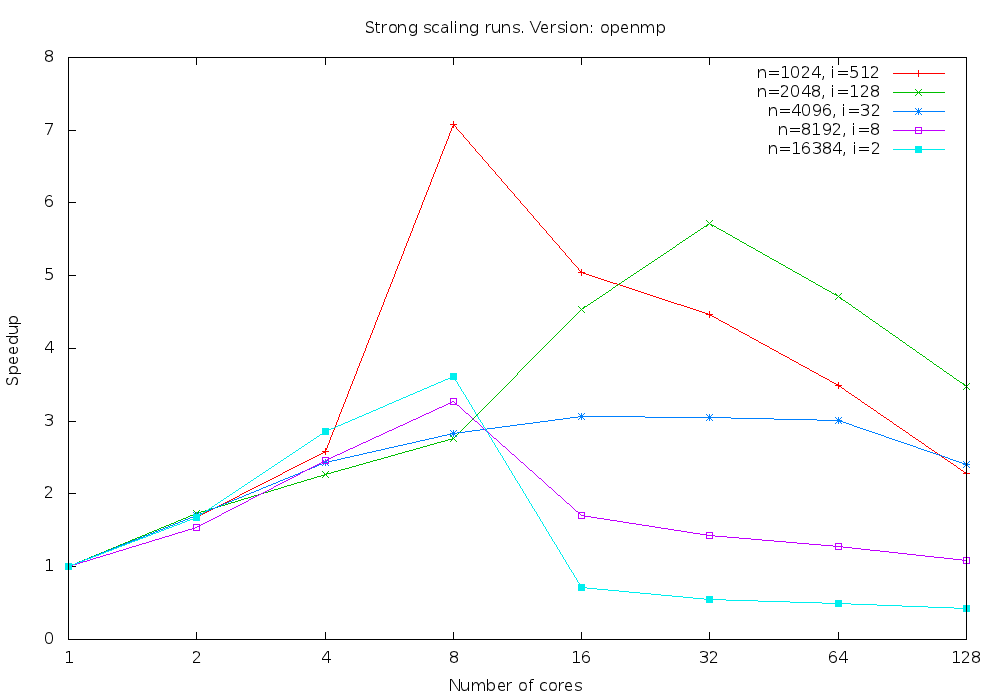
\includegraphics[width=\textwidth]{gfx/padding_strong_scaling_openmp_speedup}
\end{figure}
\end{frame}

\begin{frame}
\frametitle{First results - OpenMP (Weak scaling)}
\begin{figure}
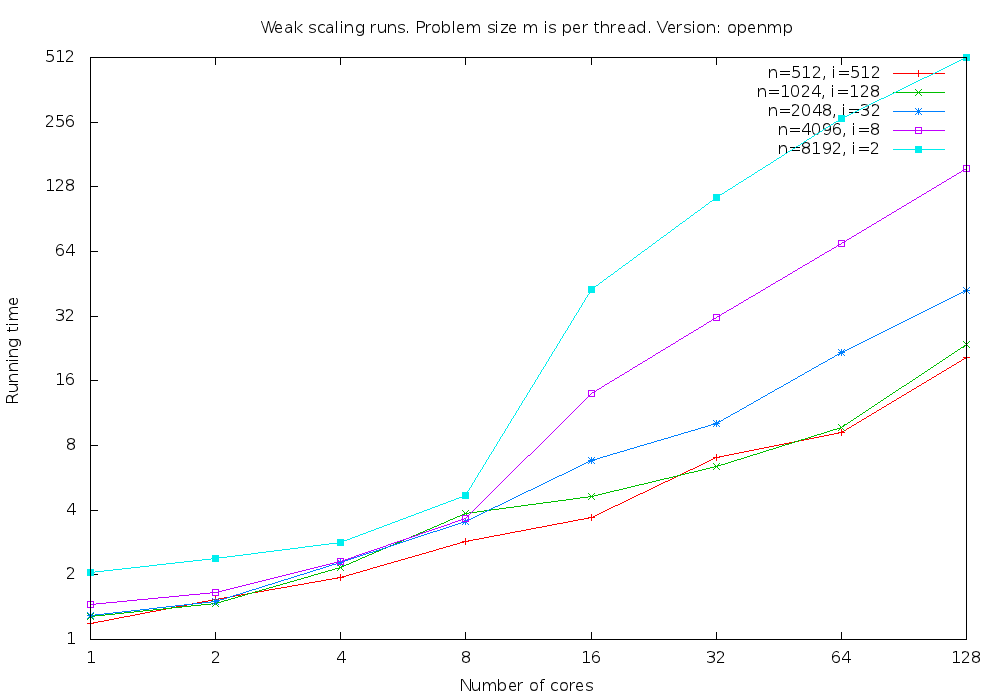
\includegraphics[width=\textwidth]{gfx/padding_weak_scaling_openmp_runningtime}
\end{figure}
\end{frame}

\begin{frame}
\frametitle{First results - Pthreads (Strong scaling)}
\begin{figure}
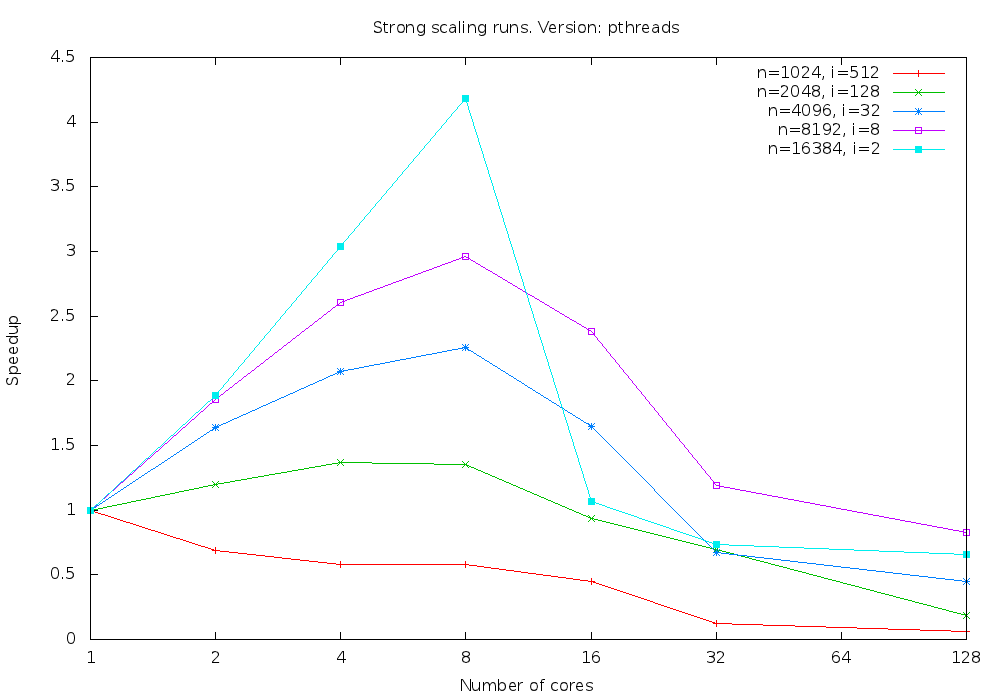
\includegraphics[width=\textwidth]{gfx/padding_strong_scaling_pthreads_speedup}
\end{figure}
\end{frame}

\begin{frame}
\frametitle{First results - Pthreads (Weak scaling)}
\begin{figure}
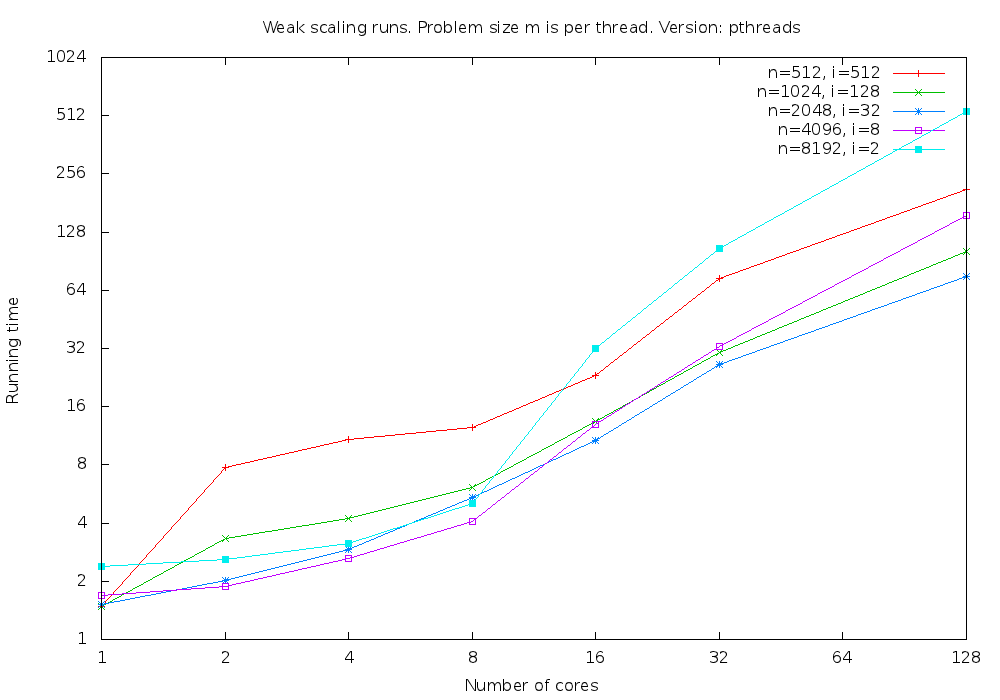
\includegraphics[width=\textwidth]{gfx/padding_weak_scaling_pthreads_runningtime}
\end{figure}
\end{frame}

\begin{frame}
\frametitle{First results}
Both implementations show the same trend.
\pause
\begin{itemize}
\item Once we go beyond one node, performance drops considerably.
\pause
\item Only exception: Mid-sized problems ($n=2048$ and $n=4096$) for OpenMP (though still horrible performance; 0.09 GFLOPS/s per core)
\item What's happening?
\end{itemize}

\pause
Possible explainations: Mid-sized problems are large enough to speed up slightly without causing too much communication overhead.
\pause

$1024^2$ is too small; For $4096^2$, communication is too expensive (?)
\end{frame}

\begin{frame}
\frametitle{Second attempt}
I partitioned the data into separate partitions with multiple malloc()s.
\pause
I let each processor initialize its own partition. This should cause that processor to "own" the data.
\pause

More explicit data motion between processors, so it's easier to see what's going on.
\end{frame}

\begin{frame}
\frametitle{Second set of results - OpenMP}
\begin{figure}
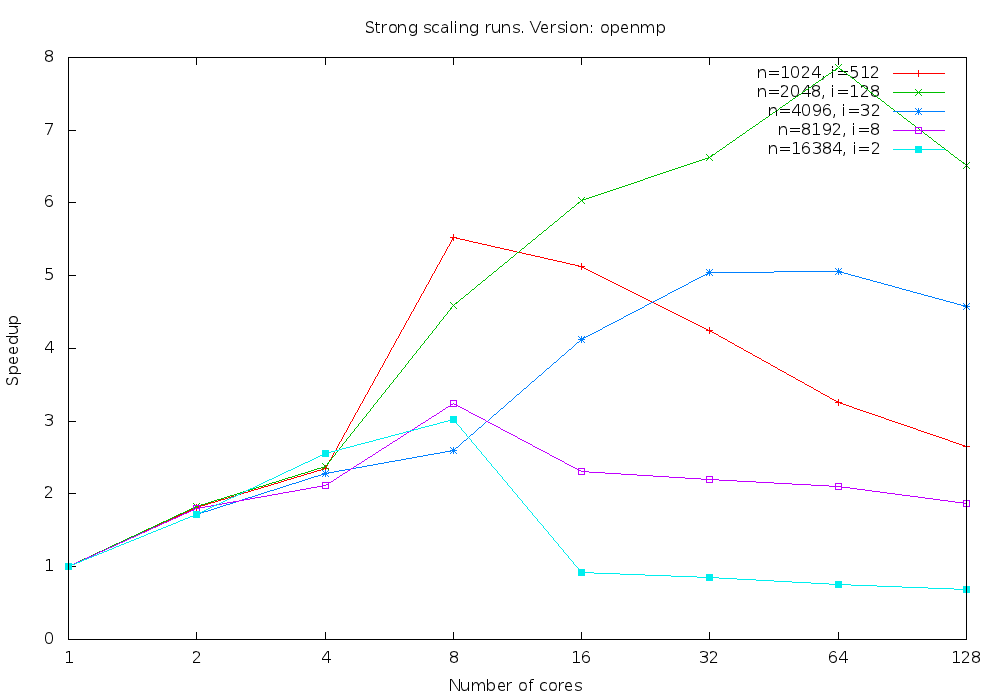
\includegraphics[width=\textwidth]{gfx/partitions_strong_scaling_openmp_speedup}
\end{figure}
\end{frame}

\begin{frame}
\frametitle{Second set of results - pthreads}
\begin{figure}
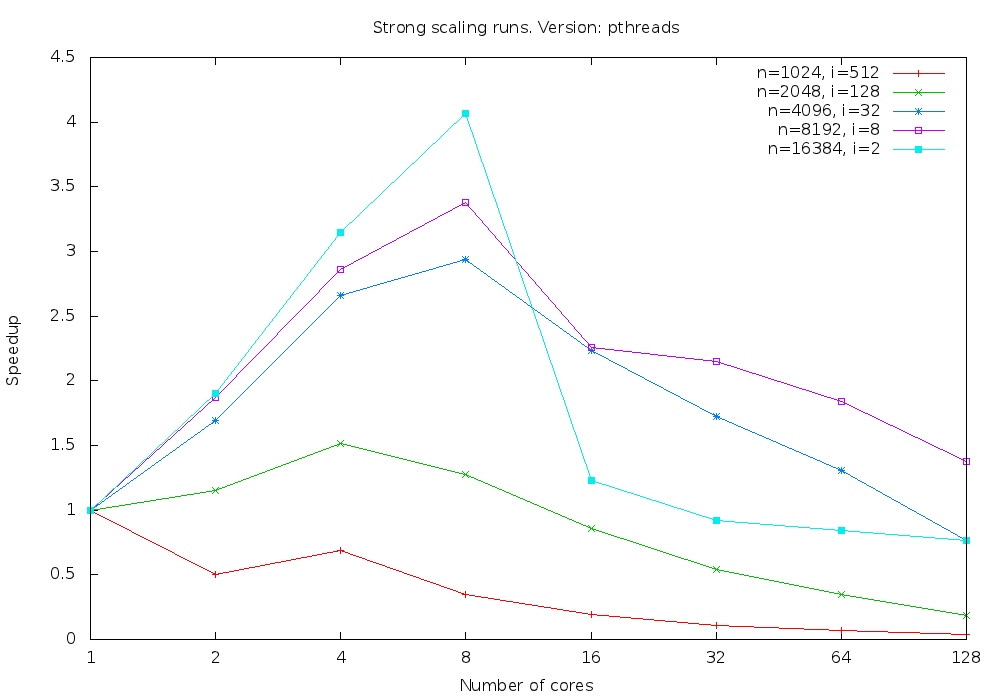
\includegraphics[width=\textwidth]{gfx/partitions_strong_scaling_pthreads_speedup}
\end{figure}
\end{frame}

\begin{frame}
\frametitle{Second set of results}
\begin{itemize}
\item Slightly better speedup for OpenMP
\pause
\item Pthreads performance still horrible
\pause
\item Still not great (about 0.15 GFLOPS per core)
\item Communication increases with the problem size 
\end{itemize}
\end{frame}

\begin{frame}
\frametitle{Next attempt: Eliminating variables}
\begin{itemize}
\item There's too many variables: Communication, synchronization,...
\pause
\item I set the problem width to a constant and disabled ghost cells and synchronization
\item No communication.
\end{itemize}
\end{frame}

\begin{frame}
\frametitle{Finally - near perfect speedup}
\begin{figure}
\includegraphics[width=\textwidth]{gfx/partitions_constant_width_nosync_strong_scaling_pthreads_noghost_speedup}
\end{figure}
\end{frame}

\begin{frame}
\frametitle{With only synchronization, no ghost cells}
\begin{figure}
\includegraphics[width=\textwidth]{gfx/partitions_constant_width_strong_scaling_pthreads_noghost_speedup}
\end{figure}
\end{frame}

\begin{frame}
\frametitle{With only ghost cells, no synchronization}
\begin{figure}
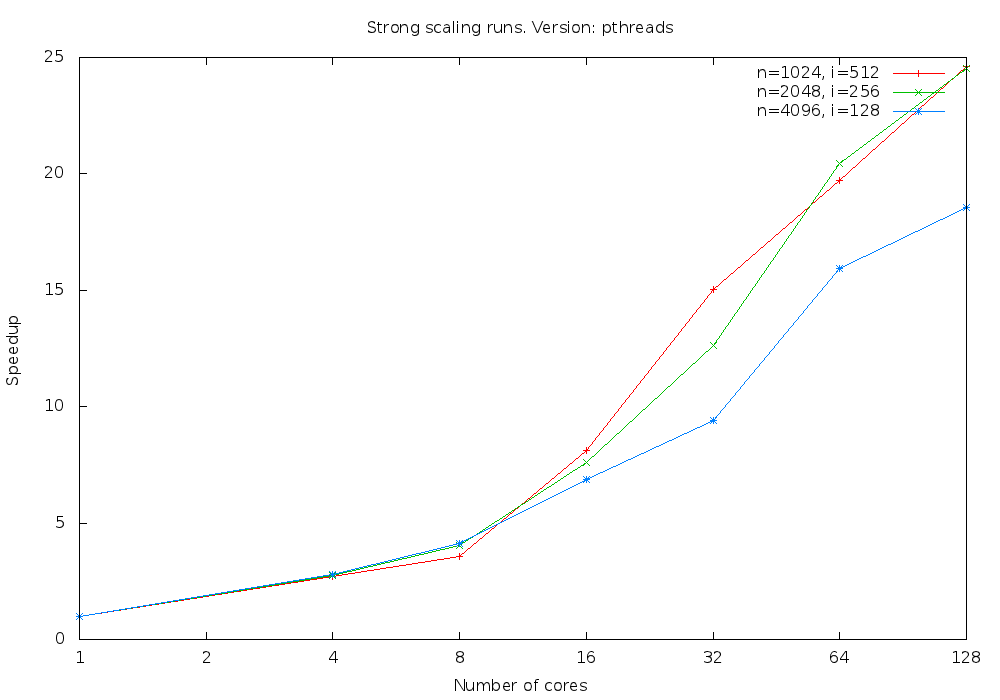
\includegraphics[width=\textwidth]{gfx/partitions_constant_width_nosync_strong_scaling_pthreads_speedup}
\end{figure}
\end{frame}

\begin{frame}
\frametitle{Observations}
\begin{itemize}
\item Communication is definitely an issue.
\pause 
\item Synchronization is a killer. Very fine grained communication, pthreads and openmp barrier not neccesarily NUMA-aware, and certainly not aware of huge page sizes
\pause
\item Without synchronization: 0.3 GFLOPS / core (getting there)
\pause
\item In short, we need a new barrier.
\end{itemize}
\end{frame}

\begin{frame}
\frametitle{Tournament barrier}
I implemented the tournament barrier.
\begin{itemize}
\item Tree-based barrier.
\pause 
\item Each node has two children.
\pause
\item Each node represents a round in a "game" where one processor is the "winner" (goes up the tree) and the other one is a "loser" (spins on a global release flag that is set by the winner of the final round).
\pause
\item Winner in each round is predetermined.
\end{itemize}
\end{frame}

\begin{frame}
\frametitle{Tournament barrier}
\begin{figure}
\includegraphics[width=\textwidth]{gfx/tournament}
\end{figure}
\end{frame}

\begin{frame}
\frametitle{Tournament barrier}
This implementation is "Dash aware" (takes large pages into consideration, and is NUMA aware)
\begin{itemize}
\item For each barrier call, variables are written to by the same processors.
\pause
\item Each processor caches a copy of the release flag. When the release flag is set by the winner, each processor fetches it again.
\pause
\item All nodes of the tree are allocated aligned to the 4K boundary to prevent false sharing.
\end{itemize}
\end{frame}

\begin{frame}
\frametitle{Results - speedup (strong scaling)}
\begin{figure}
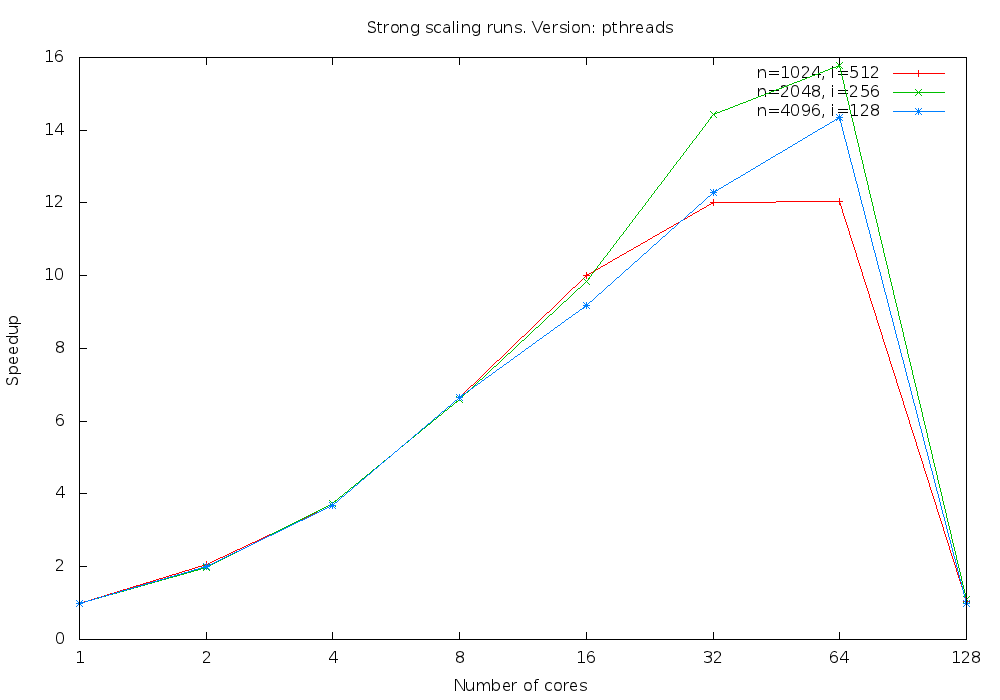
\includegraphics[width=\textwidth]{gfx/partitions_constant_width_tournament_barrier_strong_scaling_pthreads_speedup}
\end{figure}
\end{frame}

\begin{frame}
\frametitle{Results - running time (weak scaling)}
\begin{figure}
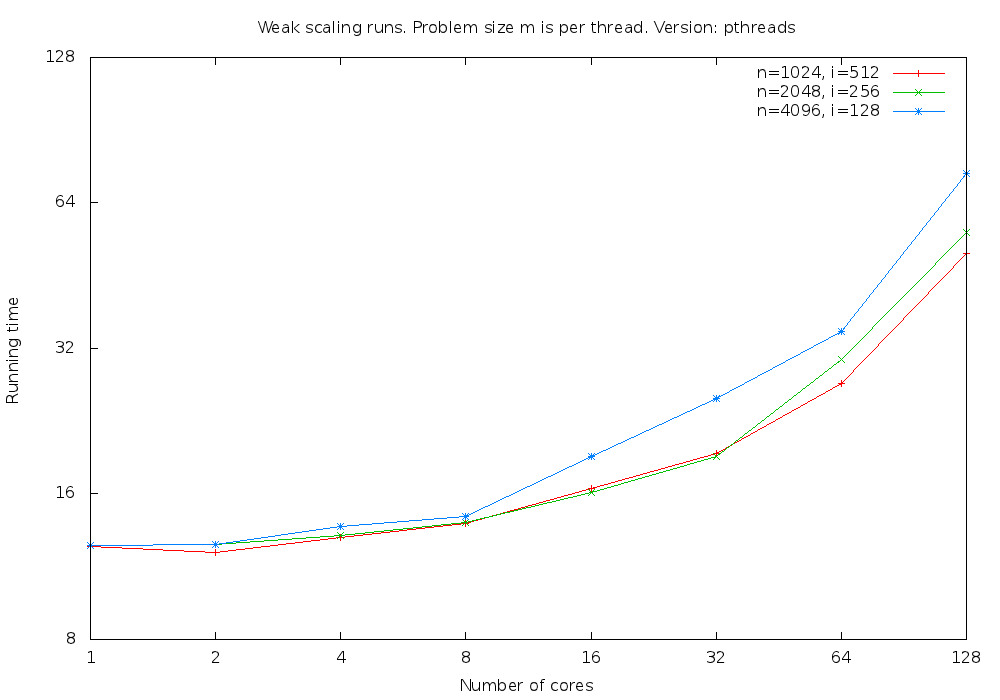
\includegraphics[width=\textwidth]{gfx/partitions_constant_width_tournament_barrier_weak_scaling_pthreads_runningtime}
\end{figure}
\end{frame}

\begin{frame}
\frametitle{Results}
\begin{itemize}
\item At 128 processors, it breaks down (still too much communication?)
\pause
\item About 0.28 GFLOPS/core for 64 cores. Barrier much less dominant.
\pause
\item The performance is (unfortunately) still bad.
\end{itemize}
\end{frame}

\begin{frame}
\frametitle{Conclusion}
\begin{itemize}
\item Synchronization on Dash is seemingly costly.
\pause
\item Barriers uses fine grained messages; Dash' pages are 4K.
\pause
\item Implementing a new barrier helped but breaks down at 128 cores.
\end{itemize}
\end{frame}

\end{document}

